% Create a Table of Contents in Beamer
\documentclass[10pt,t]{beamer}
% Theme choice:
\usetheme{Singapore}
\usecolortheme{whale}
\setbeamercolor{titlelike}{fg=blue,bg=white}
\setbeamercolor{frametitle}{fg=blue,bg=white}
\setbeamertemplate{frametitle}[default][left]
\setbeamertemplate{navigation symbols}{}

\usepackage{graphicx}
\usepackage{amsmath}
\usepackage{amsfonts}
\usepackage{amssymb}
\usepackage{amsthm}

% Title page details: 
\title{Introduction to BIOST 311} 
\author{Taylor Okonek \& Charlie Wolock}
\date{\today}



\begin{document}
	% Title page frame
	\begin{frame}
	\titlepage 
\end{frame}
% Outline frame
\begin{frame}{Outline}
\tableofcontents
\end{frame}

\AtBeginSection[ ]
{
\begin{frame}{Outline}
\tableofcontents[currentsection]
\end{frame}
}

% Presentation structure
\section{Syllabus}

\begin{frame}{Instructors}

\begin{figure}
	\begin{center}
		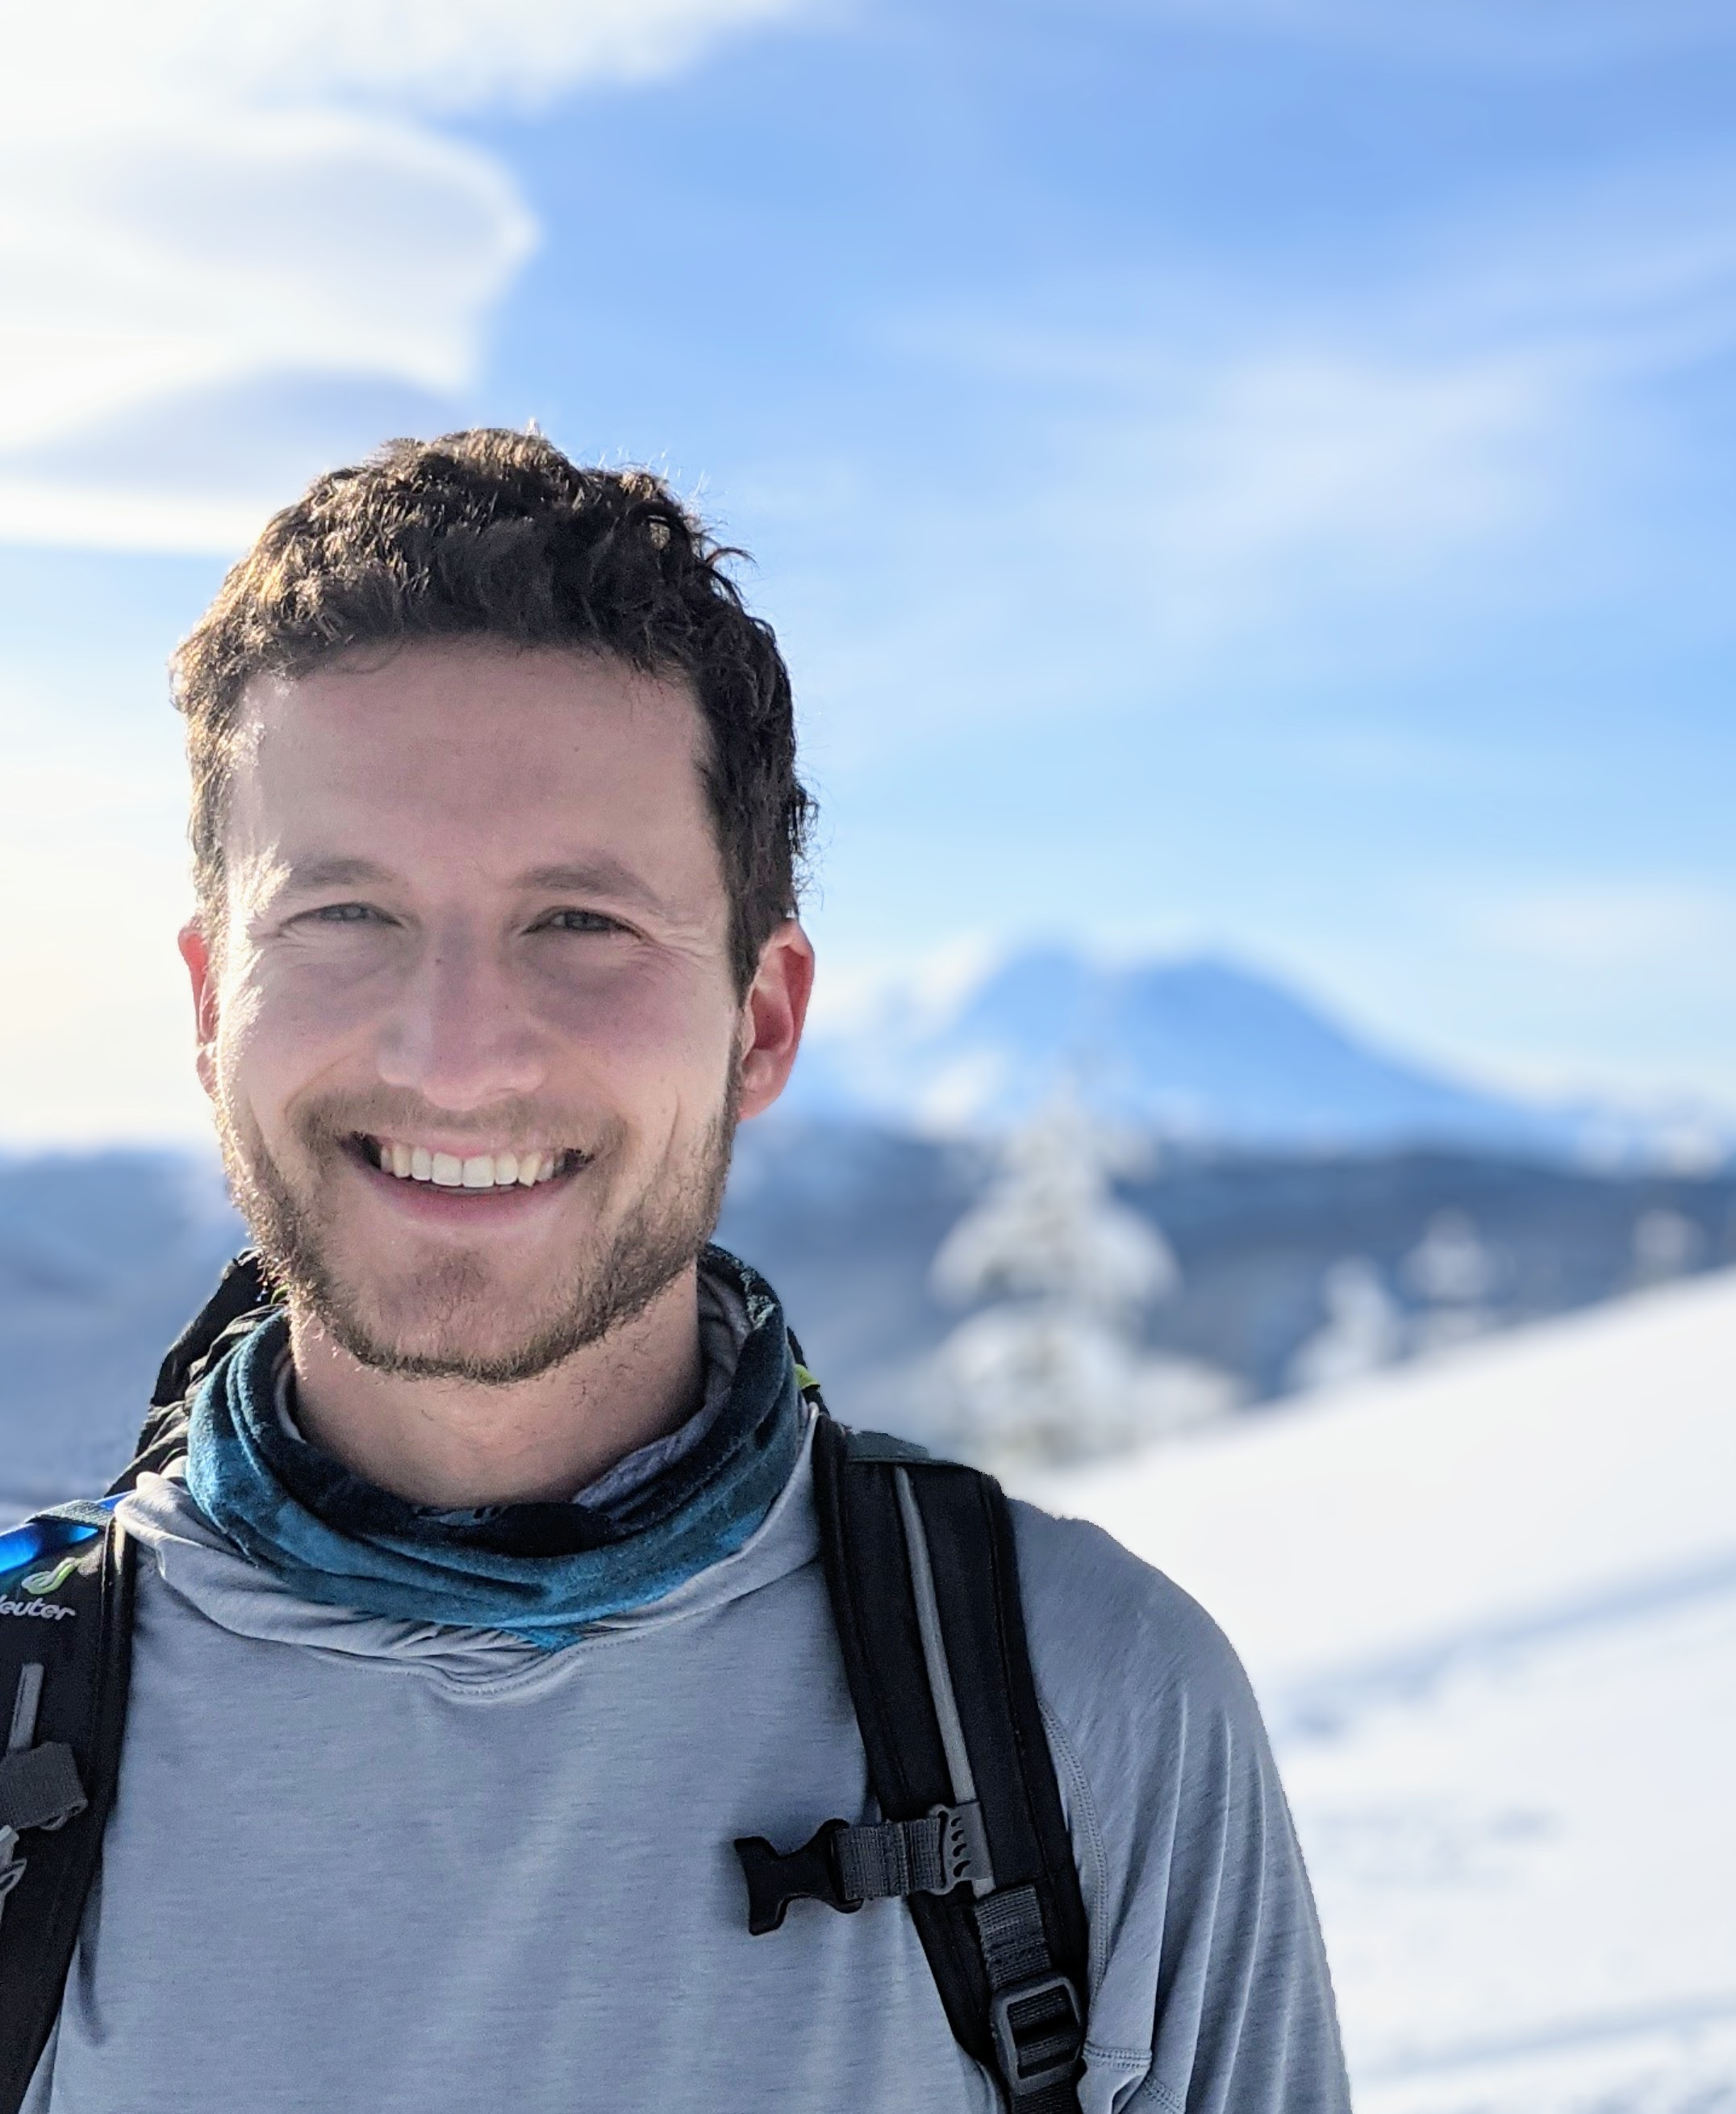
\includegraphics[height=0.4\textheight]{charlie.jpg} 
		\hspace{2cm}
		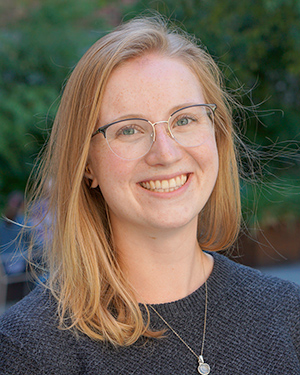
\includegraphics[height=0.4\textheight]{taylor.jpg}
	\end{center}
\end{figure}

\begin{columns}
	\begin{column}[t]{0.4\textwidth}
            \small Charlie Wolock (he/him) \\ 
            cwolock@uw.edu \\~\
            
            \small 4th year Ph.D. Student, Dept. of Biostatistics \\
            \small Statistical interests: Nonparametrics, survival analysis
	\end{column}
	\begin{column}[t]{0.4\textwidth}  %%<--- here
			\small Taylor Okonek (she/her) \\
			tokonek@uw.edu  \\~\ 
			
			\small 4th year Ph.D. Student, Dept. of Biostatistics \\
			\small Statistical interests: spatial stats, infectious disease
	\end{column}
\end{columns}

\end{frame}

\begin{frame}{Course description}
``Introduction to regression methods for analysis of continuous, binary, and time-to-event (survival) data. Covers linear regression, logistic regression, and proportional hazards regression, all at an introductory level. Makes use of examples drawn from the biomedical and health sciences literature." \\~\

\begin{itemize}
	\item Graded, 4 credits
	\item Course website: canvas.uw.edu
	\item No textbooks for the course, all material needed for homeworks/project can be found in lecture and discussion section slides
\end{itemize}

\end{frame}

\begin{frame}{Logistics}
Class sessions times and room (if not on zoom) \\
Office hours times and room (if not on zoom)
\end{frame}

\begin{frame}{Learning objectives}
\begin{itemize}
	\item Interpret numerical and graphical summaries of data that are relevant to medical and health sciences studies
	\item Interpret coefficients in linear, logistic, and proportional hazards regression models in the context of health outcomes
	\item 
Select an appropriate regression model based on a scientific question and study design
	\item Describe the necessary assumptions for linear, logistic, and proportional hazards regression in the contexts of estimation and prediction
	\item Develop and interpret confidence intervals for model parameters
	\item Set up and carry out appropriate hypothesis tests for linear, logistic, and proportional hazards regression models
	
\end{itemize}
\end{frame}

\begin{frame}{Learning objectives (continued)}
\begin{itemize}
	\item Use linear and logistic regression models to make predictions
	\item Use diagnostic procedures and sensitivity analyses to investigate potential deviations from model assumptions
	\item Use the statistical software R to:
	\begin{itemize}
		\item Read in data files
		\item Calculate summary statistics and create appropriate graphical displays
		\item Perform basic statistical inference procedures
		\item Fit linear, logistic, and proportional hazards regression models
	\end{itemize}
\end{itemize}
\end{frame}

\begin{frame}{Class communication}
We will communicate with you outside of class using the Canvas page, so please sign up to receive email notifications for the page. \\~\

Questions about course context or homework assignments should be posted to the Canvas Discussion Board, \textbf{not sent via email}. We will monitor the discussion board regularly, and also strongly encourage you to reply to each other’s questions. Concerns of a personal nature can be communicated with us via email, and in general any emails should be sent to both instructors. \\~\

Please communicate respectfully to your classmates and to us, and let us know if there are ways classroom communication can be made more accessible to you. \\~\

Instructors will not send same-day responses to messages sent after 8:00pm PST.
\end{frame}

\begin{frame}{Homework}

Homework assignments will be posted on the Canvas website one week 
prior to the due date. They should be completed in a Word or .pdf document and 
submitted electronically to the Canvas website by the due date. You are welcome to work together on homework; however, your submitted assignment (including R code, if applicable) should be in your own words. \\~\

Solution keys and individual feedback will be provided. \textcolor{red}{We have prepared a guide for how to present your assignments which is available on our Canvas page.} The lowest homework score will be dropped.

\end{frame}

\begin{frame}{Homework: Late policy}
Throughout the quarter, you may use up to three homework 
extension days. These three days may be divided up for homework assignments however you choose (for example: all three days for a single assignment, one day each for three separate assignments). \\~\

In order to use your extension days, \textbf{you must email both instructors prior to the homework due date} to inform them you plan to use an extension day. If you do not email the instructors prior to homework due date, the extension days will not be counted, and your homework will be counted as late. \\~\

Late homework receives no credit.

\end{frame}

\begin{frame}{Quizzes}
There will be weekly, open-note Canvas quizzes on Mondays. These quizzes are designed to ensure that you keep up with course material and can recall material from previous weeks. Each quiz will consist of 10 questions, 3 of which will be on information from previous weeks, and 7 of which will be on material from the most recent week of lectures. Questions will be a mix of multiple choice, True/False, and open response. \\~\

Quizzes will be graded Monday evening, and you will have 48 hours from Monday 11:59pm PST to Wednesday 11:59pm PST to complete quiz revisions, for the opportunity to earn back up to 50\% of the points you missed.
\end{frame}


\begin{frame}{Discussion section}
Discussion sections will consist of \textcolor{red}{group activities}, review of class material, discussion of group projects, and practice using R. You will be required to hand in a brief exercise (credit/no credit) at each discussion section. Your discussion section score will be based on completion of these assignments. To receive full credit for discussion section, you can miss at most one of the discussions.
\end{frame}

\begin{frame}{Final Project}
There will be a final data analysis project for which you will be given a dataset (or select your own, with approval from the instructors) and asked to develop a appropriate analysis plan, carry out the analysis, and write a short report. Projects will be introduced in the first discussion section. \textcolor{red}{You will complete your project in small groups, assigned by the instructors.}
\end{frame}

\begin{frame}{Grading}
\begin{columns}
	\begin{column}[t]{0.4\textwidth}
		Homework \\
		Quizzes \\
		Final Project \\
		Discussion Section 
	\end{column}
	\begin{column}[t]{0.4\textwidth}  %%<--- here
		30\% \\
		30\% \\
		30\% \\
		10\% 
	\end{column}
\end{columns}

\vspace{1cm}

At the end of the course, we will convert your percentage to the UW 0.0-4.0 scale. Final course grades will be calculated based on the guidelines linked below. At minimum, you will get an A (3.9-4.0) if you earn at least 95\% of the total possible points, an A- (3.5-3.8) if you earn between 90\% and 95\% of the total possible points, and a C- (1.5-1.8) if you earn 65\% of the total possible points. \\~\

Guidelines: http://depts.washington.edu/grading/practices/guidelines.html 

\end{frame}

\begin{frame}{Course policies}
\begin{itemize}
	\item \textbf{Laptops}: You will be expected to have access to a laptop during discussion sections. However, you will not generally need access to a computer during lecture (different if zoom, obviously).
	\item \textbf{Computing}: Computing in R is an important component of this course. FIND OUT WHERE THEY CAN BORROW COMPUTERS and include here. Please see us if this expectation will cause trouble for you, and we can work out a solution.
\end{itemize}
\end{frame}

\begin{frame}{Course policies (continued)}
\begin{itemize}
	\item \textbf{Collaboration}: You are encouraged to work together on homework assignments, but the final write-up should be done individually. The course project will be a \textcolor{red}{group project}; you will discuss approaches to the project with your group and other classmates during discussion sections, but outside of class you may only discuss your project with your group members and the instructors.
	\item \textbf{Academic Honesty}: Students are encouraged to familiarize themselves with the academic honesty policies. If you hand in work that is not written in your own words, you will at minimum lose all credit for the problem, and at maximum all credit for the assignment. Issues surrounding academic integrity will be handled in accordance with university policies.
\end{itemize}
\end{frame}

\begin{frame}{Course policies (continued)}
\begin{itemize}
	\item \textbf{Grading}: We will have assignments graded in a timely fashion. If you have questions or concerns about the grading, see us. We reserve the right to change or not change the grade.
\end{itemize}
\end{frame}

\begin{frame}{Classroom climate}
The UW School of Public Health seeks to ensure all students are fully included in each course. We strive to create an environment that reflects community and mutual caring. We encourage students with concerns about classroom climate to talk to your instructor, your advisor, a member of the departmental or SPH Diversity Committee and/or the program director. DCinfo@uw.edu is a resource for students with classroom climate concerns.
\end{frame}

\begin{frame}{Concerns}
If you have any concerns about the class or your instructors, please feel free to talk to or email us at any time during the quarter. If you are not comfortable talking with us or not satisfied with the response that you receive, you may contact the Department of Biostatistics Associate Director of Academic Affairs (biostgp@uw.edu). If you still are not satisfied with the response, you may contact the Department of Biostatistics Chair (bchair@uw.edu). You may also contact the Graduate School at G-1 Communications Building, by phone at 206-543-5139 or by email at raan@uw.edu.
\end{frame}

\begin{frame}{Academic integrity}
Students at the University of Washington (UW) are expected to maintain the highest standards of academic conduct, professional honesty, and personal integrity.
 \\~\

The UW School of Public Health (SPH) is committed to upholding standards of academic integrity consistent with the academic and professional communities of which it is a part. Plagiarism, cheating, and other misconduct are serious violations of the University of Washington Student Conduct Code (WAC 478-121). We expect you to know and follow the university’s policies on cheating and plagiarism, and the SPH Academic Integrity Policy. Any suspected cases of academic misconduct will be handled according to University of Washington regulations. For more information, see the University of Washington Community Standards and Student Conduct website.

\end{frame}

\begin{frame}{Access and accommodation}
\small Your experience in this class is important to us. If you have already established accommodations with Disability Resources for Students (DRS), please communicate your approved accommodations to us at your earliest convenience so we can discuss your needs in this course.
\\~\

\small If you have not yet established services through DRS, but have a temporary health condition or permanent disability that requires accommodations (conditions include but not limited to; mental health, attention-related, learning, vision, hearing, physical or health impacts), you are welcome to contact DRS at 206-543- 8924 or uwdrs@uw.edu or disability.uw.edu. DRS offers resources and coordinates reasonable accommodations for students with disabilities and/or temporary health conditions. Reasonable accommodations are established through an interactive process between you, your instructor(s) and DRS. It is the policy and practice of the University of Washington to create inclusive and accessible learning environments consistent with federal and state law.

\end{frame}

\begin{frame}{First Canvas quiz!}
Please complete the Canvas quiz by Friday! \textcolor{red}{tbd a bit, but we should do something like this probably} 

\vspace{0.3cm}

\begin{itemize}
	\item Name
	\item Pronunciation guide
	\item What are you most looking forward to learning this quarter?
	\item What do you anticipate having the most trouble with this quarter?
\end{itemize}

\vspace{0.3cm}

Pronunciation guide example:
\begin{itemize}
	\item Taylor Okonek
	\item TAY-lor AH-ke-nik
\end{itemize}

\vspace{0.3cm}

\color{blue} We'll do a mid-quarter Stop/Start/Continue check-in as well!

\end{frame}

\begin{frame}{What to Expect: Statistics}
You will need light algebra and mathematical reasoning
\vspace{0.3cm}
\begin{itemize}
	\item No calculus assumed
	\item We won't prove technical results, but can provide resources for those available if asked
	\item Quizzes will not require any math beyond basic arithmetic, and are open note
\end{itemize}

\vspace{0.3cm}

This course is the natural sequel to BIOST 310 

\vspace{0.3cm}

We will learn how to build regression models, estimate parameters, and interpret coefficients 

\vspace{0.3cm}

Examples will be primarily in public health or health sciences applications

\end{frame}

\begin{frame}{What to Expect: Computing}
We will learn basic statistical computing in \texttt{R}

\vspace{0.3cm}

You are \textit{not} expected to have a computing background

\vspace{0.3cm}

\begin{itemize}
	\item We will demonstrate important functions in lectures and discussion sections
	\item We will provide helpful resources: templates for homework assignments, \texttt{R} code "cheat sheets" with useful functions, video tutorials (as applicable), etc. \textcolor{red}{We need to make cheat sheets i guess}
\end{itemize}

\vspace{0.3cm}

\textbf{Homework for tonight:} download \texttt{R} and \texttt{R Studio} (see instructions on Canvas) \textcolor{red}{need to make instructions}

\end{frame}

\begin{frame}[c]
\centering \huge Any Questions?
\end{frame}

\section{Motivation}

\begin{frame}{Why is statistics important?}
\begin{itemize}
	\item We have a research question we want to answer
	\item We hear a claim we think is false, and want to refute it
	\item We have a \textit{ton} of information and we don't know how to make sense of it
	\item We understand the current state of things, but want to predict future outcomes
\end{itemize}
\end{frame}

\begin{frame}{Example: Research question}

Retinol (a Vitamin A derivative) is a popular skin care agent that has been shown in studies to decrease wrinkle surface area and hyperpigmentation. However, retinol is not safe to use for pregant individuals, and additionally retinol has known side-effects of causing skin dryness and stinging for many people. Bakuchiol has been proposed as a retinol alternative that is safe for pregnant individuals to use and does not have similar negative side-effects. However, we are not sure if Bakuchiol is \textit{as effective} as retinol for decreasing wrinkle surface area and hyperpigmentation. 

\vspace{0.3cm}

Q: \textit{Is Bakuchiol as effective as retinol for improving wrinkle surface area and hyperpigmentation?} 

\vspace{0.3cm}

How do we answer this question? (one option: \href{https://onlinelibrary.wiley.com/doi/10.1111/bjd.16918}{a randomized trial})

\end{frame}

\begin{frame}{Example: Research question}

\begin{itemize}
	\item Randomly assign 44 individuals to either use Bakuchiol or Retinol over the course of 12 weeks, surveying individuals and taking images every 4 weeks 
	\item Use image analysis to determine fine wrinkle surface area at each time point
\end{itemize}

\centering 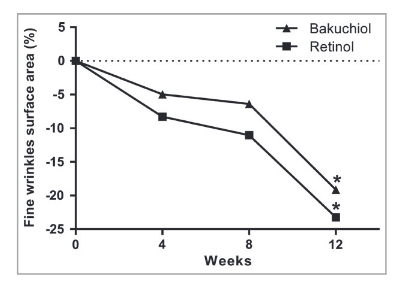
\includegraphics[scale=0.4]{retinol.png}

\end{frame}

\begin{frame}{Example: Research question}

Why is statistics important?

\vspace{0.3cm}

In this example:
\begin{itemize}
	\item Allows us to determine whether or not there is a difference in outcomes based on exposure (retinol vs. Bakuchiol) that is due to \textit{the exposure alone} (i.e. no other variable could have mattered)
	\item A standardized way of measuring the outcome. This study didn't compare qualitatively if they thought individuals had a lower wrinkle surface area, they used image analysis!
	\item Allows us to determine if there is a \textit{statistically significant} difference in outcomes between Bakuchiol and retinol users (we'll come back to this throughout the course)
\end{itemize}

\end{frame}

\begin{frame}[c]{Example: Refuting a false claim}
\centering 
\includegraphics[scale=0.4]{lancet.png}
\end{frame}

\begin{frame}{Example: Refuting a false claim}
A paper published in the Lacet (a relatively high-impact journal!) in 1998 suggested that the measles, mumps, and rubella (MMR) vaccine may cause autism spectrum disorder in children.

\centering 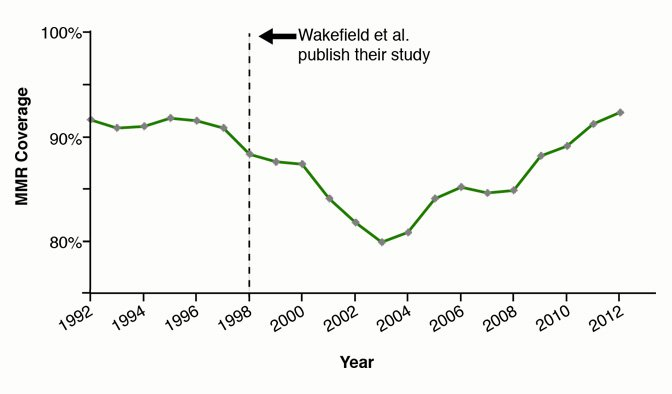
\includegraphics[scale=0.4]{mmrvax.jpg}

\end{frame}

\begin{frame}{Example: Refuting a false claim}

Statistical tools used to critically assess (and eventually refute) this claim:
\begin{itemize}
	\item The sample size in their study was $n = 12$ (which is \textit{very} small)
	\item Their study design was uncontrolled, so causal claims could not be made (more on this to follow in the Study Design review section!)
\end{itemize}

\vspace{0.3cm}

Why is statistics important?
\begin{itemize}
	\item Allows us to critically assess scientific claims
	\item Understanding the assumptions underlying statistical methods and study designs lets us think \textit{scientifically and statistically} about whether or not these assumptions are met
\end{itemize}

\vspace{0.3cm}

\footnotesize An important aside with this study is that the lead author was funded by lawyers who had been representing parents in lawsuits against vaccine-producing companies. Critically reading studies from \textit{many} angles (not only statistical) is important! A more detailed summary of this article and follow-up can be found \href{https://www.ncbi.nlm.nih.gov/pmc/articles/PMC3136032/}{\color{cyan} here}.

\end{frame}

\begin{frame}{Example: How do we make sense of data?}

\begin{itemize}
	\item Cholera outbreak in 1854 in London
	\item People were unsure where it was coming from (airborne? spread through food? from animals?)
	\item Informational available: where cholera patients lived
	\item John Snow (below) decided to make a map...
\end{itemize}

\vspace{0.3cm}

\centering 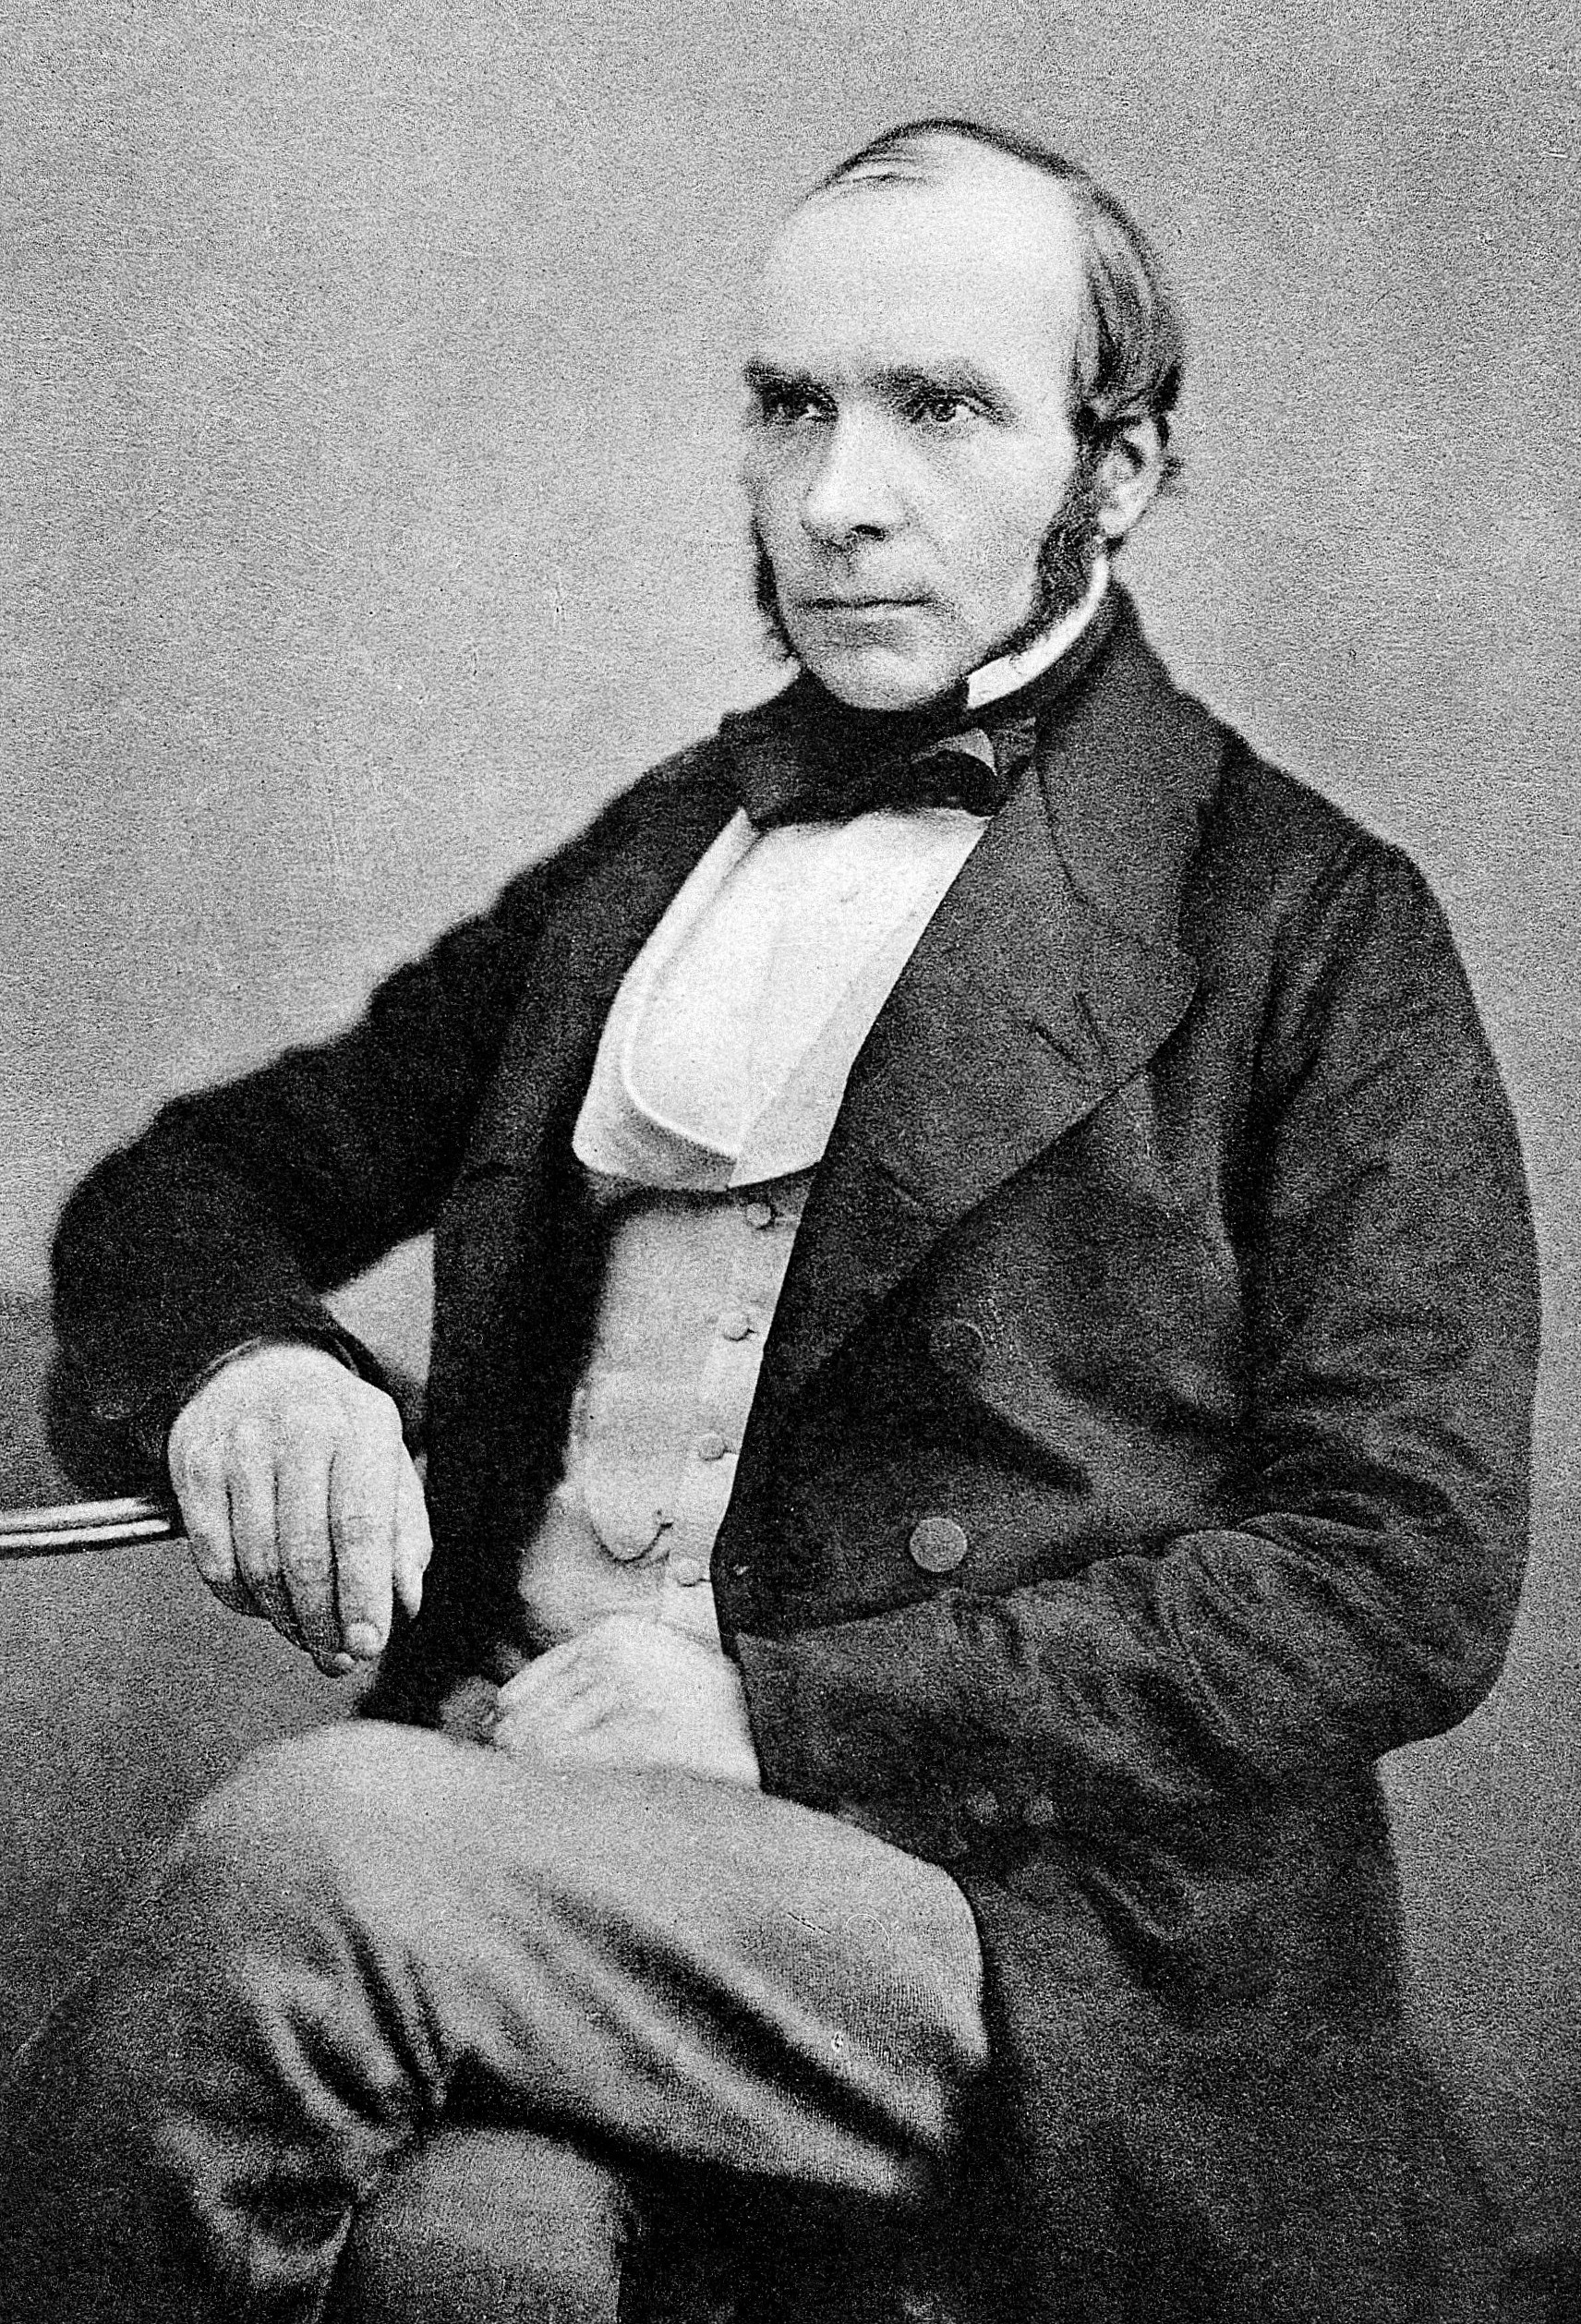
\includegraphics[scale=0.17]{johnsnow_epi.jpg} 

\end{frame}

\begin{frame}[c]{Example: How do we make sense of data?}

\centering 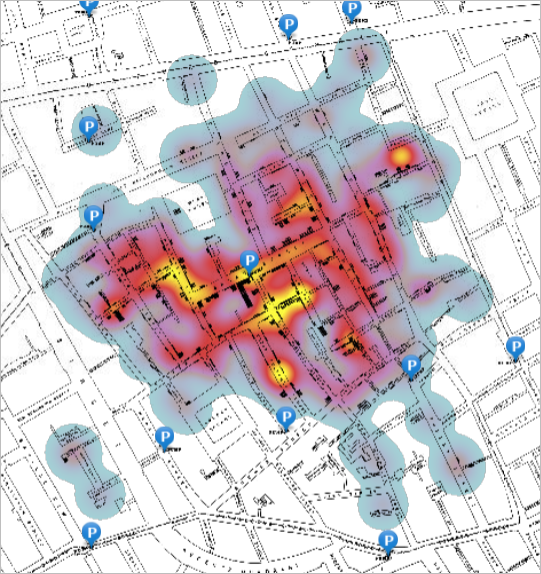
\includegraphics[scale=0.4]{cholera.png}

\end{frame}

\begin{frame}{Example: How do we make sense of data?}


\begin{itemize}
	\item Mapping the cholera cases was the key to realizing the disease was spread through water, specifically the Broad Street pump
	\item An example of descriptive spatial statistics
\end{itemize}

Why is statistics important?
\begin{itemize}
	\item Allows us to distinguish patterns in data that were previously unclear
	\item With this specific example, more advanced statistical methods could be used to detect clusters of points in space
\end{itemize}

\end{frame}

\begin{frame}[c]{Example: Prediction}
\centering 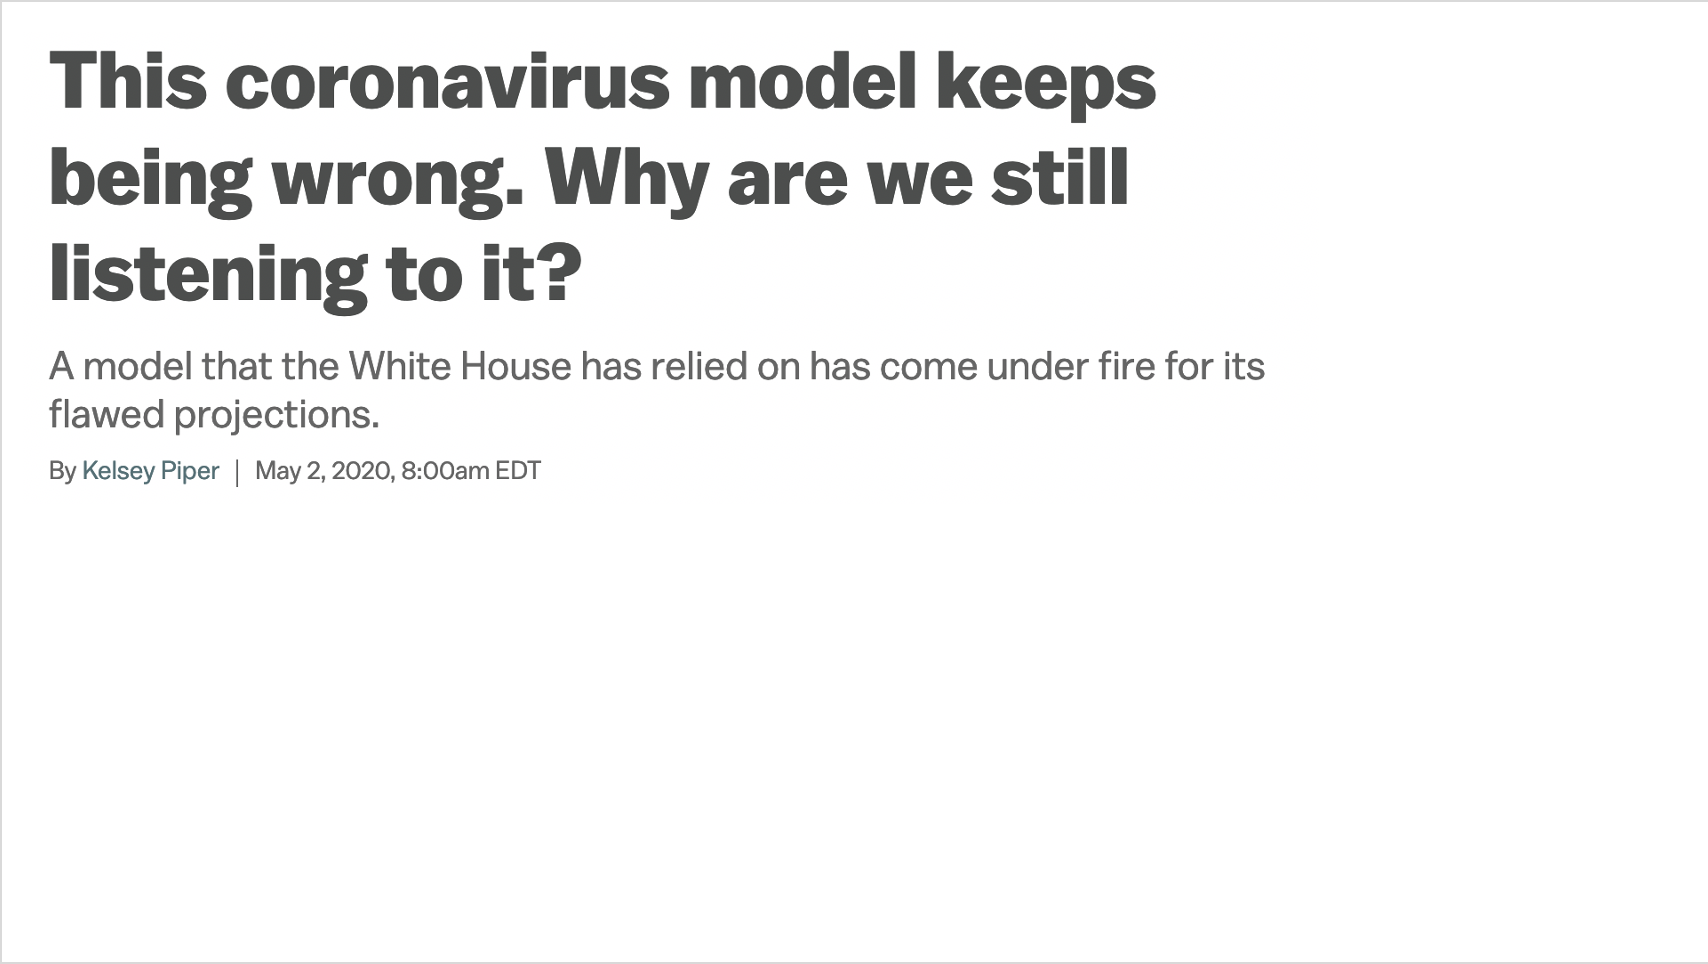
\includegraphics[scale=0.37]{ihme1.png}
\end{frame}

\begin{frame}[c]{Example: Prediction}
\centering 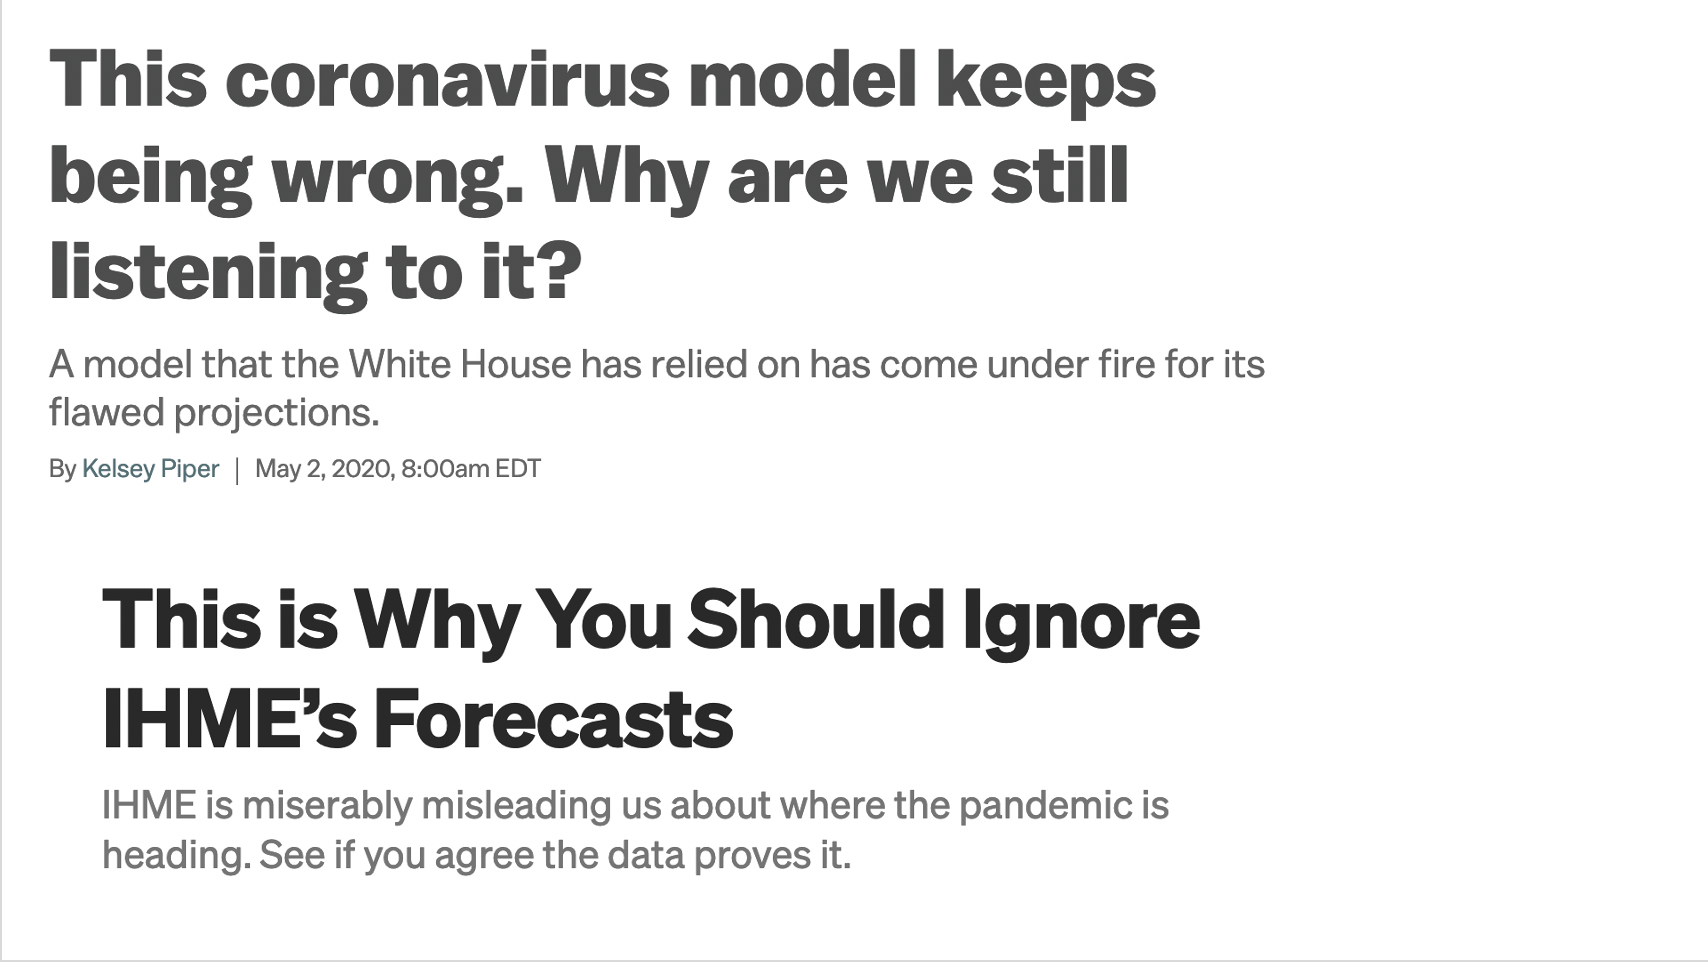
\includegraphics[scale=0.37]{ihme2.png}
\end{frame}

\begin{frame}[c]{Example: Prediction}
\centering 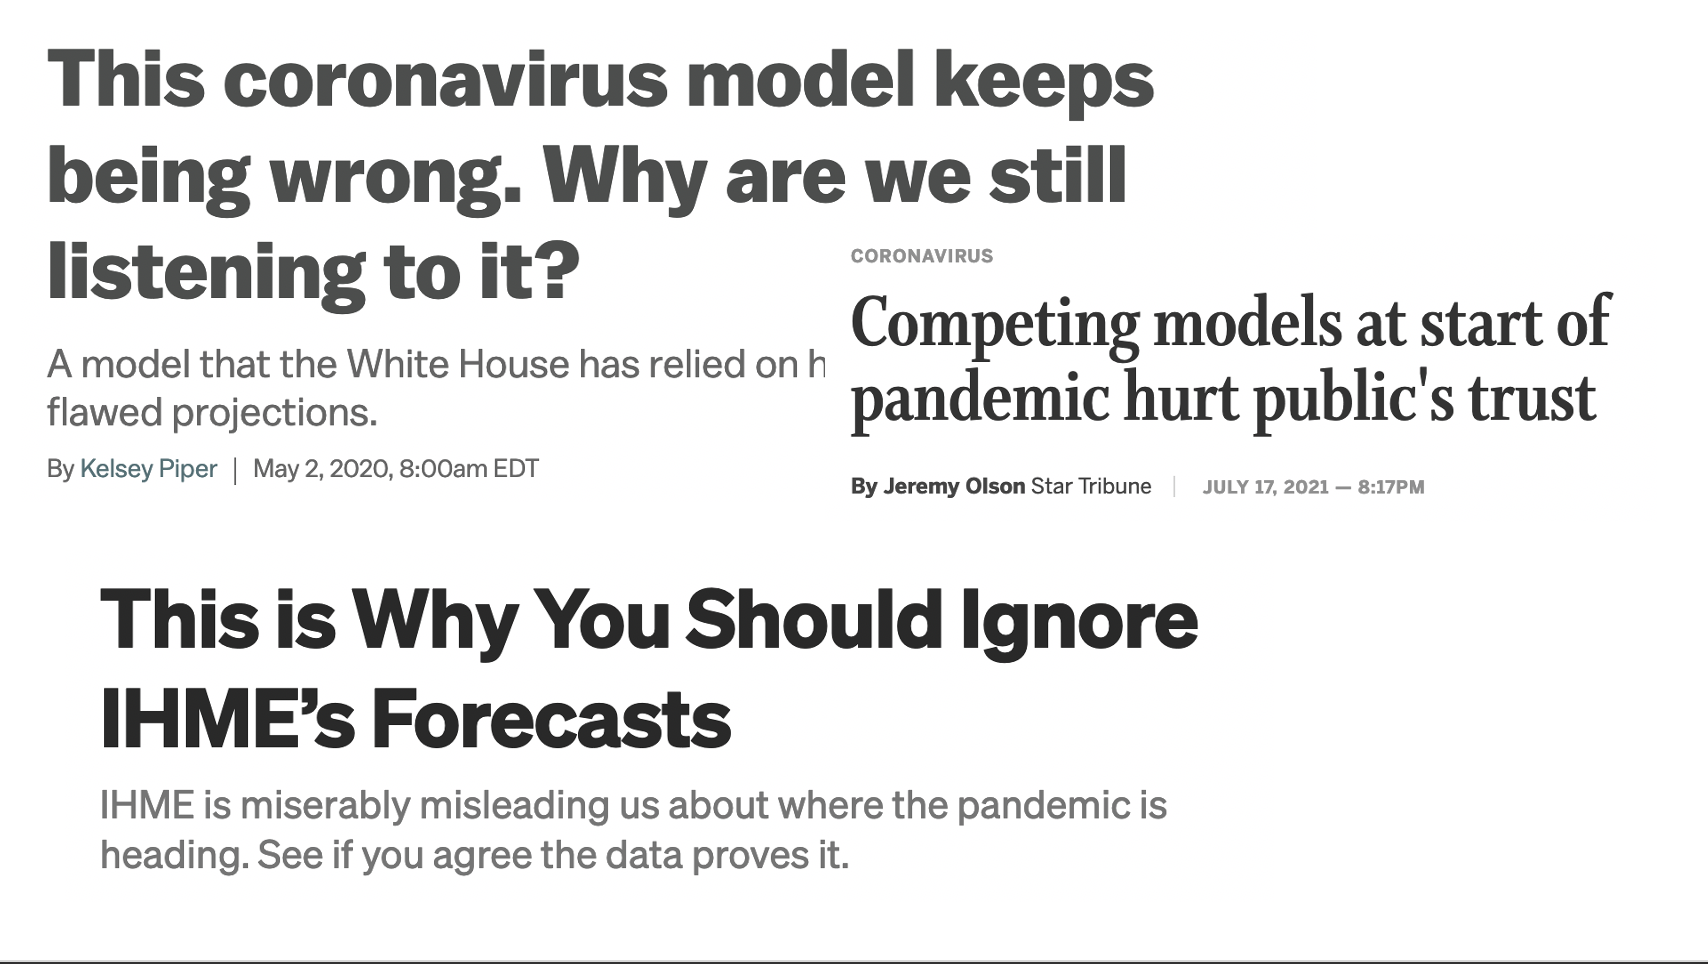
\includegraphics[scale=0.37]{ihme3.png}
\end{frame}

\begin{frame}[c]{Example: Prediction}
\centering 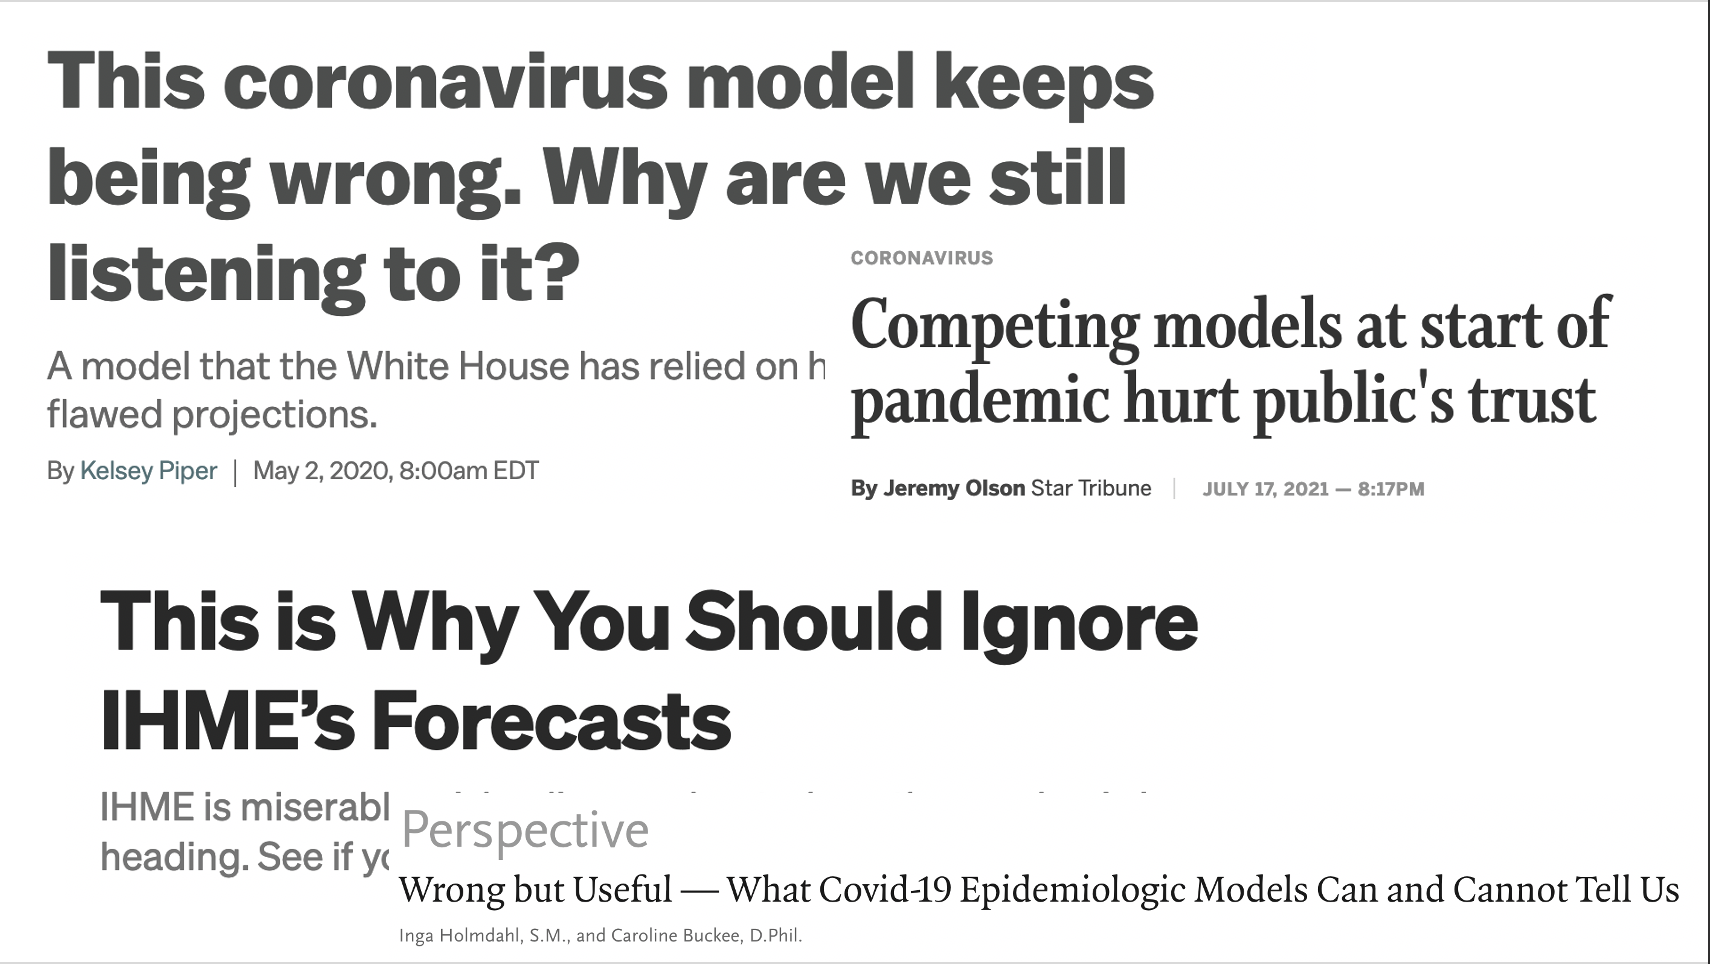
\includegraphics[scale=0.37]{ihme4.png}
\end{frame}

\begin{frame}[c]{Example: Prediction}
\centering 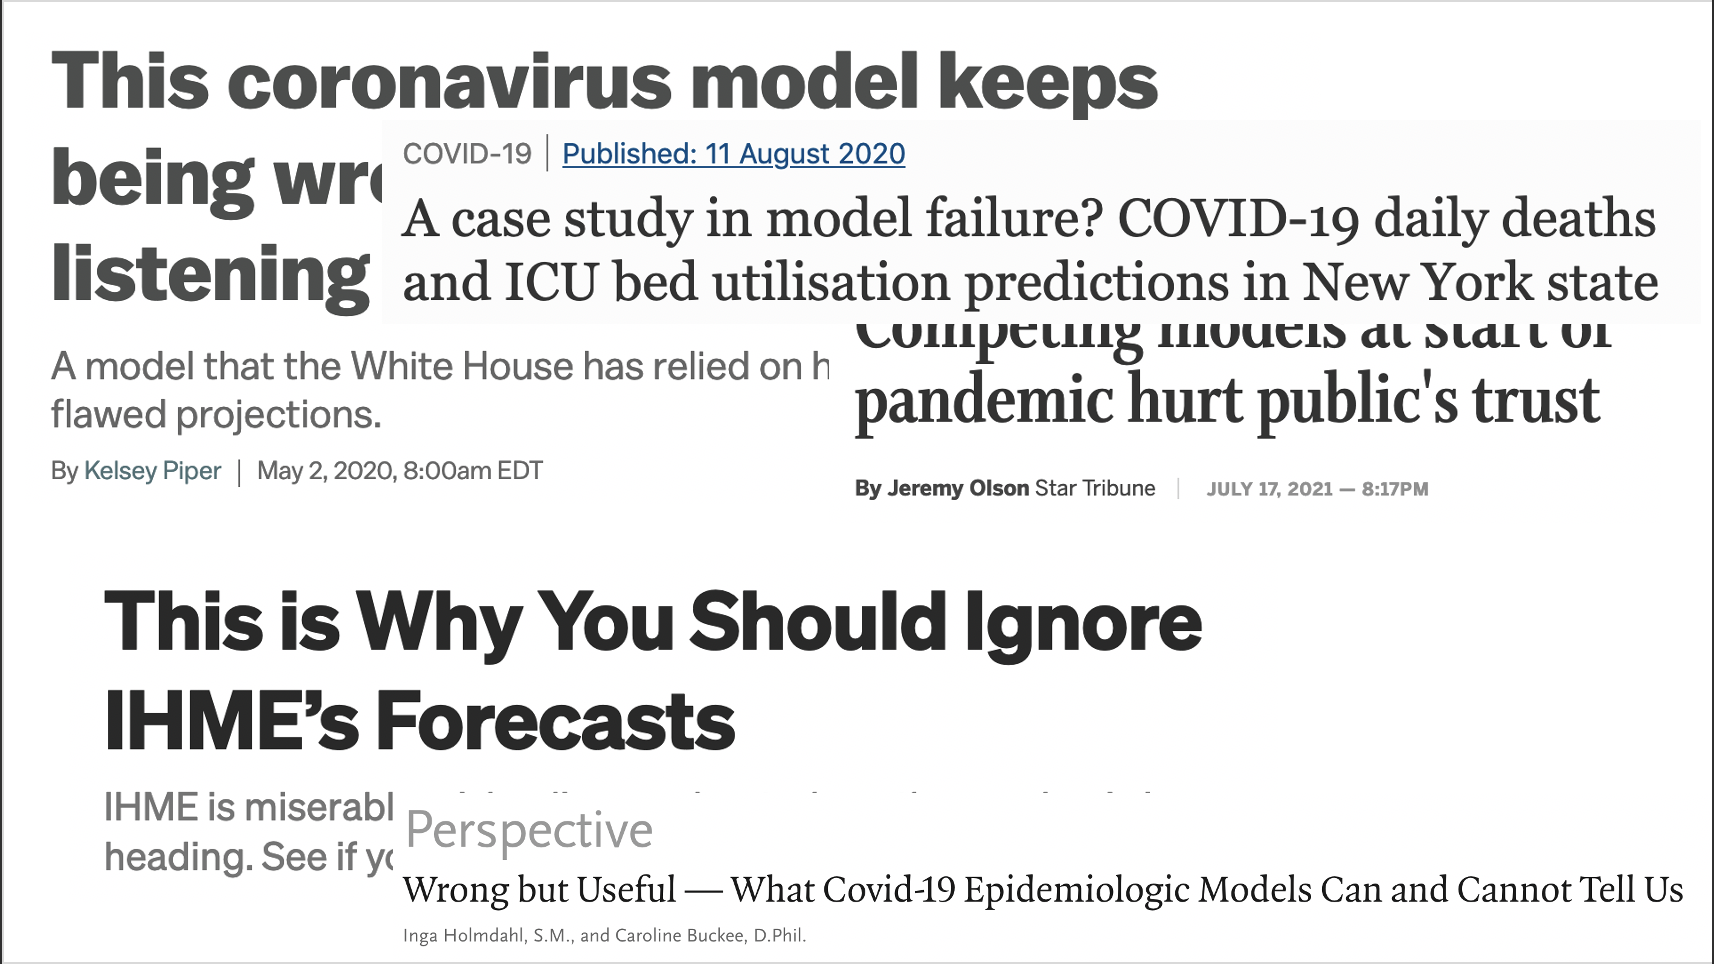
\includegraphics[scale=0.37]{ihme5.png}
\end{frame}

\begin{frame}[c]{Example: Prediction}
\centering 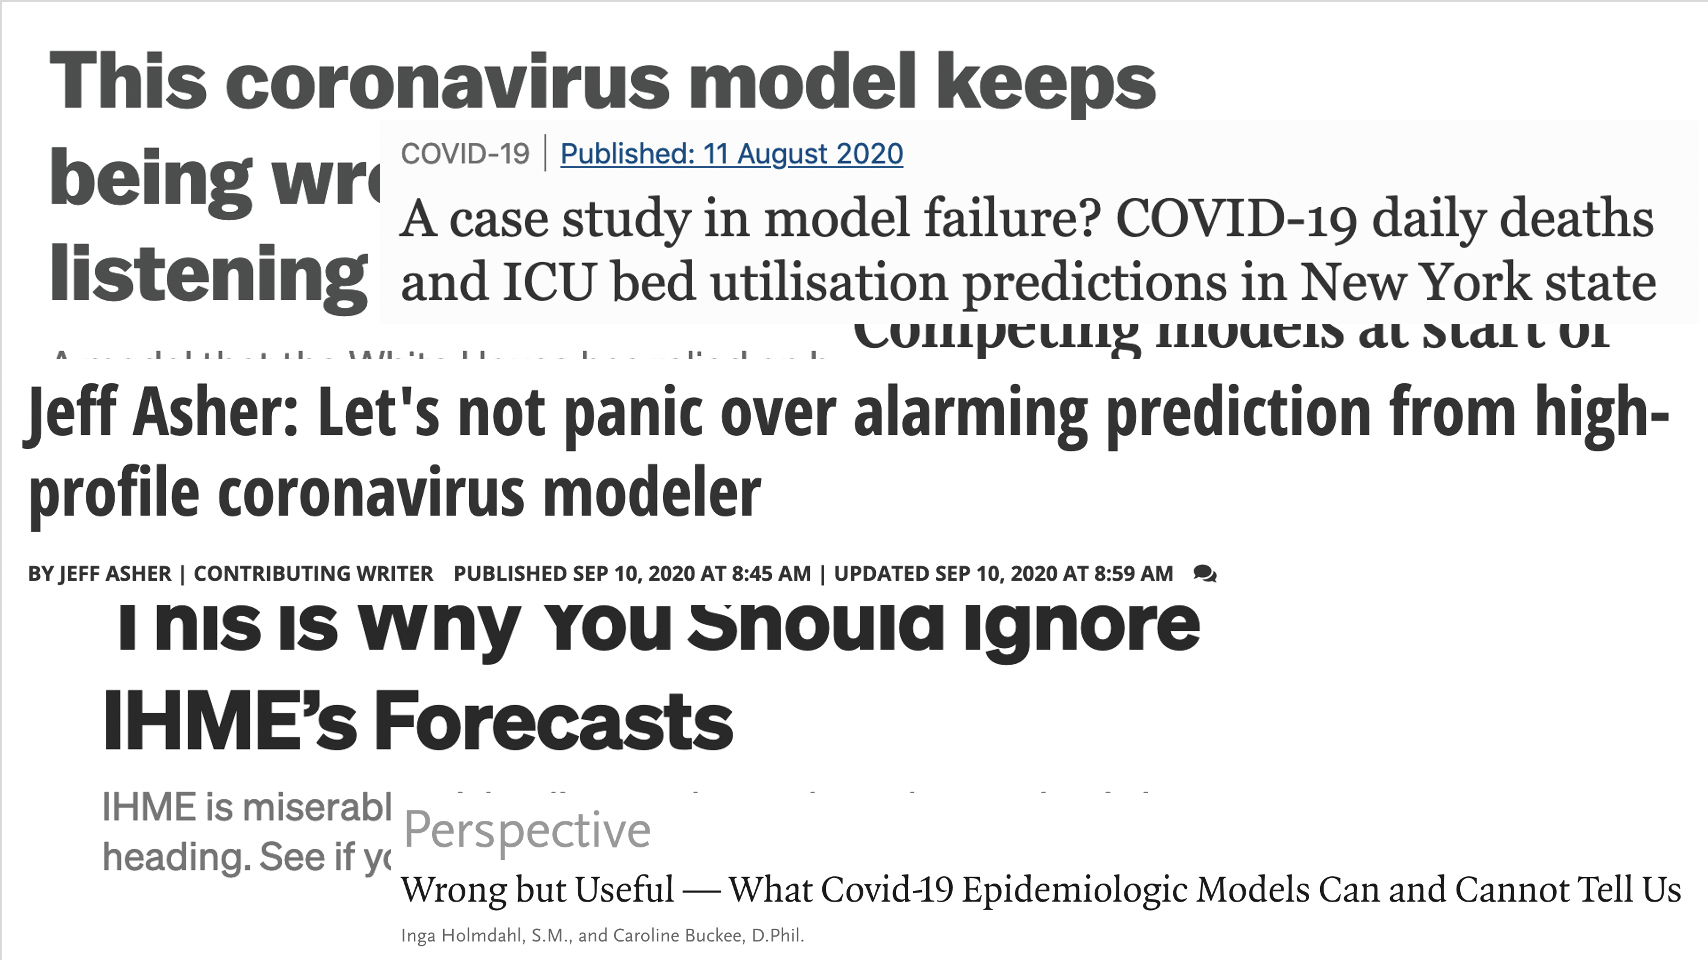
\includegraphics[scale=0.37]{ihme6.png}
\end{frame}

\begin{frame}[c]{Example: Prediction}
\centering 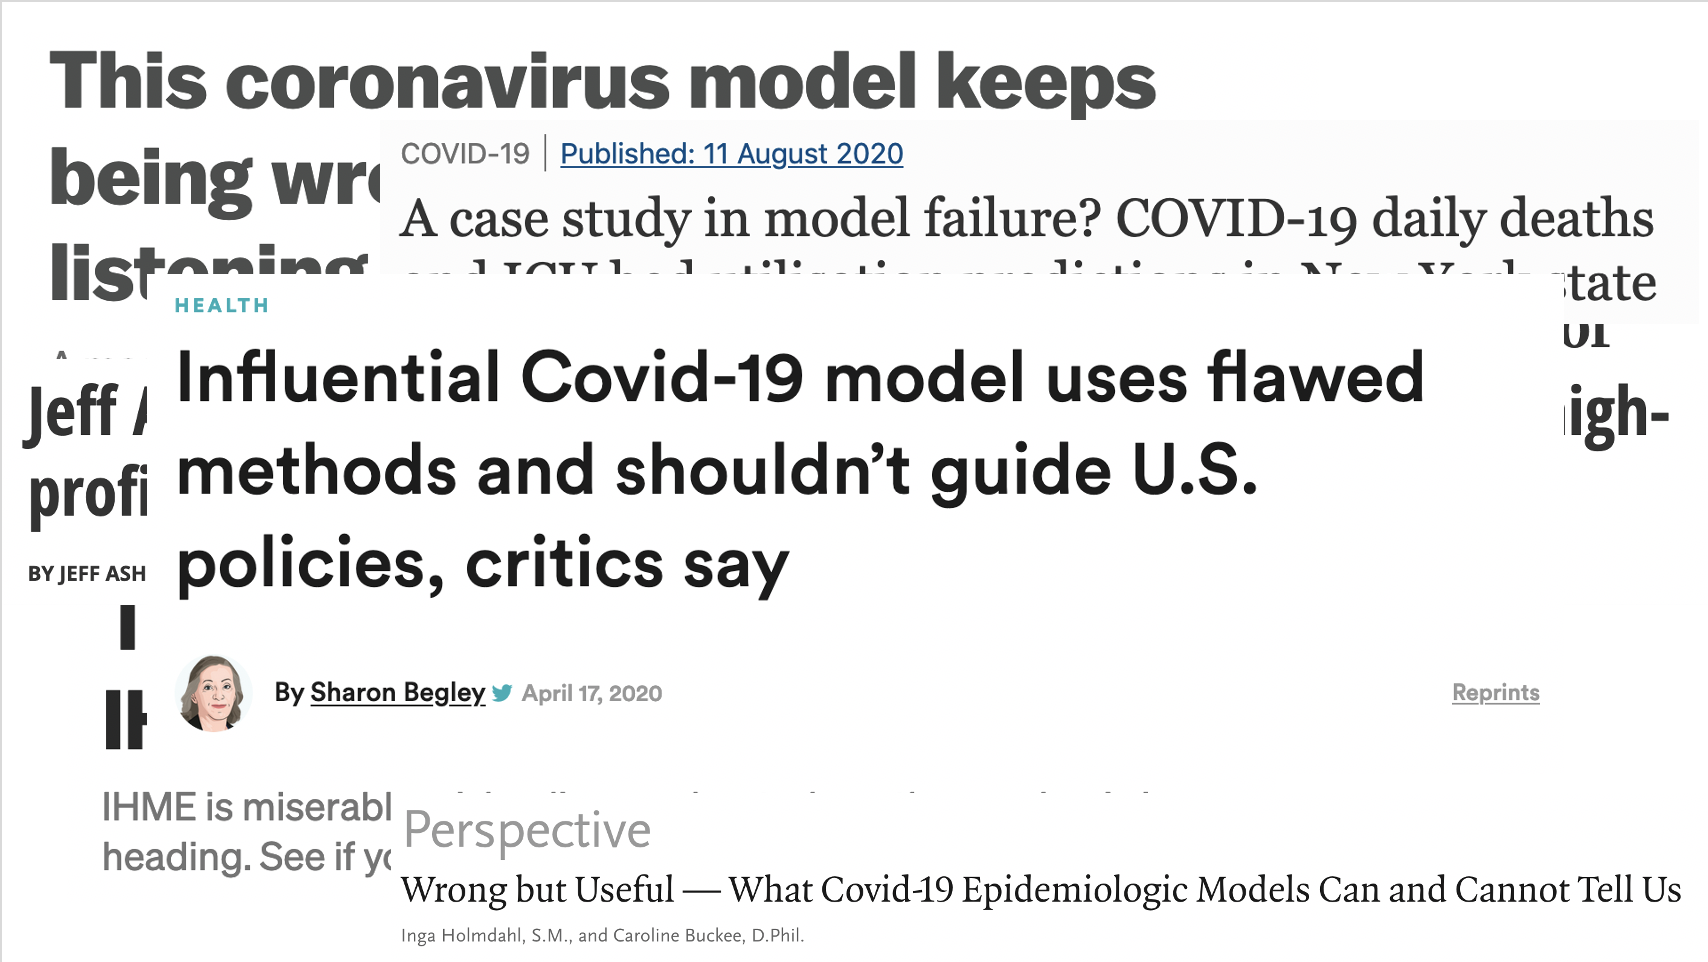
\includegraphics[scale=0.37]{ihme7.png}
\end{frame}

\begin{frame}{Example: Prediction}
Why is statistics important?
\begin{itemize}
	\item Statistics influences public policy and our daily lives
	\item Care needs to be taken when developing prediction models
	\begin{itemize}
		\item Which covariates may be important predictors of the outcome?
		\item Which covariates are extraneous and don't need to be included?
		\item Are any of the covariates we include \textit{problematic}, or may lead to conclusions that are socially unjust?
		\item What social (political) context do we need to be considering when making a prediction model?
	\end{itemize}
	\item Uncertainty needs to be appropriately calculated \textit{and} reported
\end{itemize}
\end{frame}

\begin{frame}{Key Takeaway}
Regression (the main focus of our course) is a statistical tool underlying \textit{many} statistical problems, including some of the ones we just discussed!
\end{frame}

\begin{frame}[c]
\centering \huge Any Questions?
\end{frame}

\end{document}